\documentclass{article}
\usepackage[paperwidth=275mm,paperheight=112mm,margin=0pt]{geometry}
\usepackage{tikz}
\usepackage{graphicx}
\usepackage{amsmath,amssymb}
\usepackage{xcolor}
\graphicspath{{report/image/}{image/}}
\usetikzlibrary{arrows.meta,backgrounds,calc,fit,positioning}
\pagestyle{empty}

\definecolor{panel}{HTML}{FFFFFF}
\definecolor{ink}{HTML}{30343B}
\definecolor{targetgray}{HTML}{777B82}
\definecolor{encoderfill}{HTML}{E8E1F0}
\definecolor{modelfill}{HTML}{F3DCCF}
\definecolor{bodyfill}{HTML}{DDEED6}
\definecolor{latentfill}{HTML}{E4F3FA}
\definecolor{latentblue}{HTML}{5AA9CE}
\definecolor{lossfill}{HTML}{FFFFFF}
\definecolor{emphasisred}{HTML}{D94A45}
\definecolor{bodyblue}{HTML}{DCEBFA}

\tikzset{
  font=\sffamily\footnotesize,
  >={Latex[length=2.2mm,width=1.4mm]},
  flow/.style={draw=ink, line width=.85pt, ->},
  line/.style={draw=ink, line width=.85pt},
  hotflow/.style={draw=emphasisred, line width=1.05pt, ->},
  target/.style={draw=targetgray, line width=.75pt, dashed, ->},
  model/.style={draw=ink, fill=modelfill, line width=.8pt,
    rounded corners=2.5pt, align=center, minimum width=28mm,
    minimum height=10mm, inner sep=3pt},
  hotmodel/.style={model, draw=emphasisred, line width=1.35pt},
  encoder/.style={draw=ink!75, fill=encoderfill, line width=.7pt,
    rounded corners=2pt, align=center, minimum width=22mm,
    minimum height=12mm, inner sep=2.5pt},
  bodyhead/.style={draw=emphasisred, fill=bodyfill, line width=1.35pt,
    rounded corners=2.5pt, align=center, minimum width=32mm,
    minimum height=10mm, inner sep=3pt},
  latent/.style={draw=latentblue, fill=latentfill, line width=1.1pt,
    rounded corners=3pt, align=center, minimum width=17mm,
    minimum height=9mm, inner sep=1.5pt,
    font=\sffamily\bfseries\footnotesize},
  loss/.style={draw=emphasisred, fill=lossfill, line width=1.25pt,
    rounded corners=4pt, align=center, minimum width=24mm,
    minimum height=9mm, inner sep=2pt},
  imageframe/.style={draw=emphasisred, fill=white, line width=1.2pt,
    rounded corners=1pt, inner sep=0pt},
  bodybox/.style={draw=ink, fill=bodyblue, line width=.8pt,
    rounded corners=2.5pt, align=center, minimum width=27mm,
    minimum height=11mm, inner sep=3pt},
  actionbox/.style={draw=emphasisred, fill=white, line width=1.25pt,
    rounded corners=2.5pt, align=center, minimum width=31mm,
    minimum height=10mm, inner sep=3pt},
  note/.style={fill=panel, inner sep=1pt, font=\scriptsize},
  steptag/.style={circle, draw=ink, fill=ink, text=white,
    inner sep=0pt, minimum size=4.2mm,
    font=\sffamily\bfseries\tiny}
}

\begin{document}
\thispagestyle{empty}
\vspace*{\fill}
\noindent\makebox[\paperwidth][c]{%
\begin{tikzpicture}[x=1mm,y=1mm]
  \begin{scope}[on background layer]
    \path[draw=ink!35, fill=panel, line width=.8pt, rounded corners=5pt]
      (-8,-49) rectangle (256,49);
  \end{scope}
  \node[font=\sffamily\bfseries\large, text=ink] at (124,42) {Closed-loop action selection};

  \begin{scope}[xshift=10mm]
  % ---------------------------------------------------------------------
  % Goal-video branch: infer the target Froude sequence from visual goal.
  
  \node[imageframe] (goalA) at (11,20.5)
    {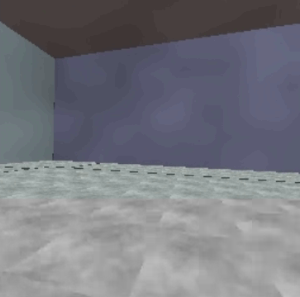
\includegraphics[width=20mm,height=14mm]{1.png}};
  \node[imageframe] (goalB) at (13,15.5)
    {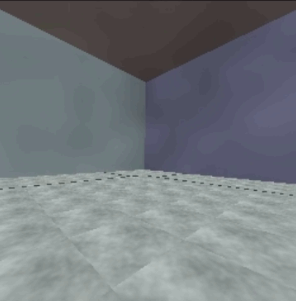
\includegraphics[width=20mm,height=14mm]{2.png}};
  \node[align=center, text=ink!80, font=\scriptsize] at (13,4.5)
    {Goal video\\window};

  \node[encoder] (enc) at (43,18) {Frozen Visual\\Encoder};
  \node[model] (itm) at (83,18) {Inverse Transition\\Model};
  \node[latent] (zg) at (115,18)
    {$z_t^g $\hspace{1.0mm}{\scriptsize\color{latentblue!85!black}$\in \mathbb{R}^{64}$}};
  \node[bodyhead] (goalhead) at (154,18) {Body-motion Head};
  \node[loss] (goalfroude) at (197,18) {goal Froude\\$\mathbf v_t^{g}$};
  \draw[flow] (18,18) -- (enc.west);
  \draw[flow] (enc) -- node[above,note] {$(e_t,e_{t+1})$} (itm);
  \draw[flow] (itm) -- (zg);
  \draw[flow] (zg) -- (goalhead);
  \draw[flow] (goalhead) -- (goalfroude);

  % ---------------------------------------------------------------------
  % Candidate-action branch: score actions by predicted body motion.
  \node[bodybox] (body) at (13,-18) {New body\\at state $s_t$};
  \node[actionbox] (candidates) at (57,-18) {Candidate actions\\$\{a_t^{(k)}\}_{k=1}^{K}$};
  \node[hotmodel, fill=latentfill, minimum width=31mm] (proj) at (103,-18) {Action Projector};
  \node[latent] (za) at (139,-18)
    {$z_t^{(k)} $\hspace{1.0mm}{\scriptsize\color{latentblue!85!black}$\in \mathbb{R}^{64}$}};
  \node[bodyhead] (predhead) at (178,-18) {Body-motion Head};
  \node[loss] (predfroude) at (220,-18) {predicted Froude\\$\hat{\mathbf v}_t^{(k)}$};

  \draw[hotflow] (body) -- (candidates);
  \draw[hotflow] (candidates) -- (proj);
  \draw[hotflow] (proj) -- (za);
  \draw[hotflow] (za) -- (predhead);
  \draw[hotflow] (predhead) -- (predfroude);

  \node[loss, minimum width=24mm] (mse) at (220,-2)
    {MSE match};
  \draw[hotflow] (goalfroude.east) -- (220,18) -- (mse.north);
  \draw[hotflow] (predfroude.north) -- (mse.south);

  \node[actionbox] (chosen) at (142,-2)
    {selected action\\$a_t^\star$};
  \draw[hotflow] (mse.west) -- (chosen.east);

  % Closed-loop rollout arrow.
  \draw[hotflow] (chosen.west) -- (13,-2) -- (body.north);
  \node[align=center, font=\scriptsize, text=emphasisred] at (73,-43)
    {execute $a_t^\star$, advance simulator/body, repeat for $t=1\dots T$};

  % Small labels for the three conceptual stages.
  \node[steptag, anchor=south west] at (itm.north west) {1};
  \node[steptag, anchor=south west] at (proj.north west) {2};
  \node[steptag, anchor=south west] at (mse.north west) {3};
  \end{scope}

  \node[font=\scriptsize, text=targetgray, anchor=east] at (252,-43)
    {red: closed-loop action-selection path};
\end{tikzpicture}%
}
\vspace*{\fill}
\end{document}
